\section{How to build an \ab{} workflow system}

\subsection{Sciency, technical stuff}

\begin{frame}{Various \ab{} software}

    To do \ab{} calculations, it is inevitable to interact with \ab{} software.
    There are a lot of software on the market, e.g., \qe{}, VASP, and ABINIT.
    They are often written in Fortran, and needed to be compiled to executable
    when using.

    So building a workflow for them requires us to create parsers for their input and output
    files, as well as functions to dynamically run these executables.

    \begin{figure}[b]
        \centering
        
\includegraphics[width=0.4\textwidth]{qe}
        \hfill
        
\includegraphics[width=0.2\textwidth]{vasp}
        \hfill
        
\includegraphics[width=0.3\textwidth]{abinit}
        \label{fig:abinitsoftware}
    \end{figure}

\end{frame}

\begin{frame}[allowframebreaks]{What does \express{} include?}

    \express{} is the workflow framework's name, including several Julia packages,
    while \texttt{Express.jl} is the core component of it.

    \begin{figure}
        \centering
        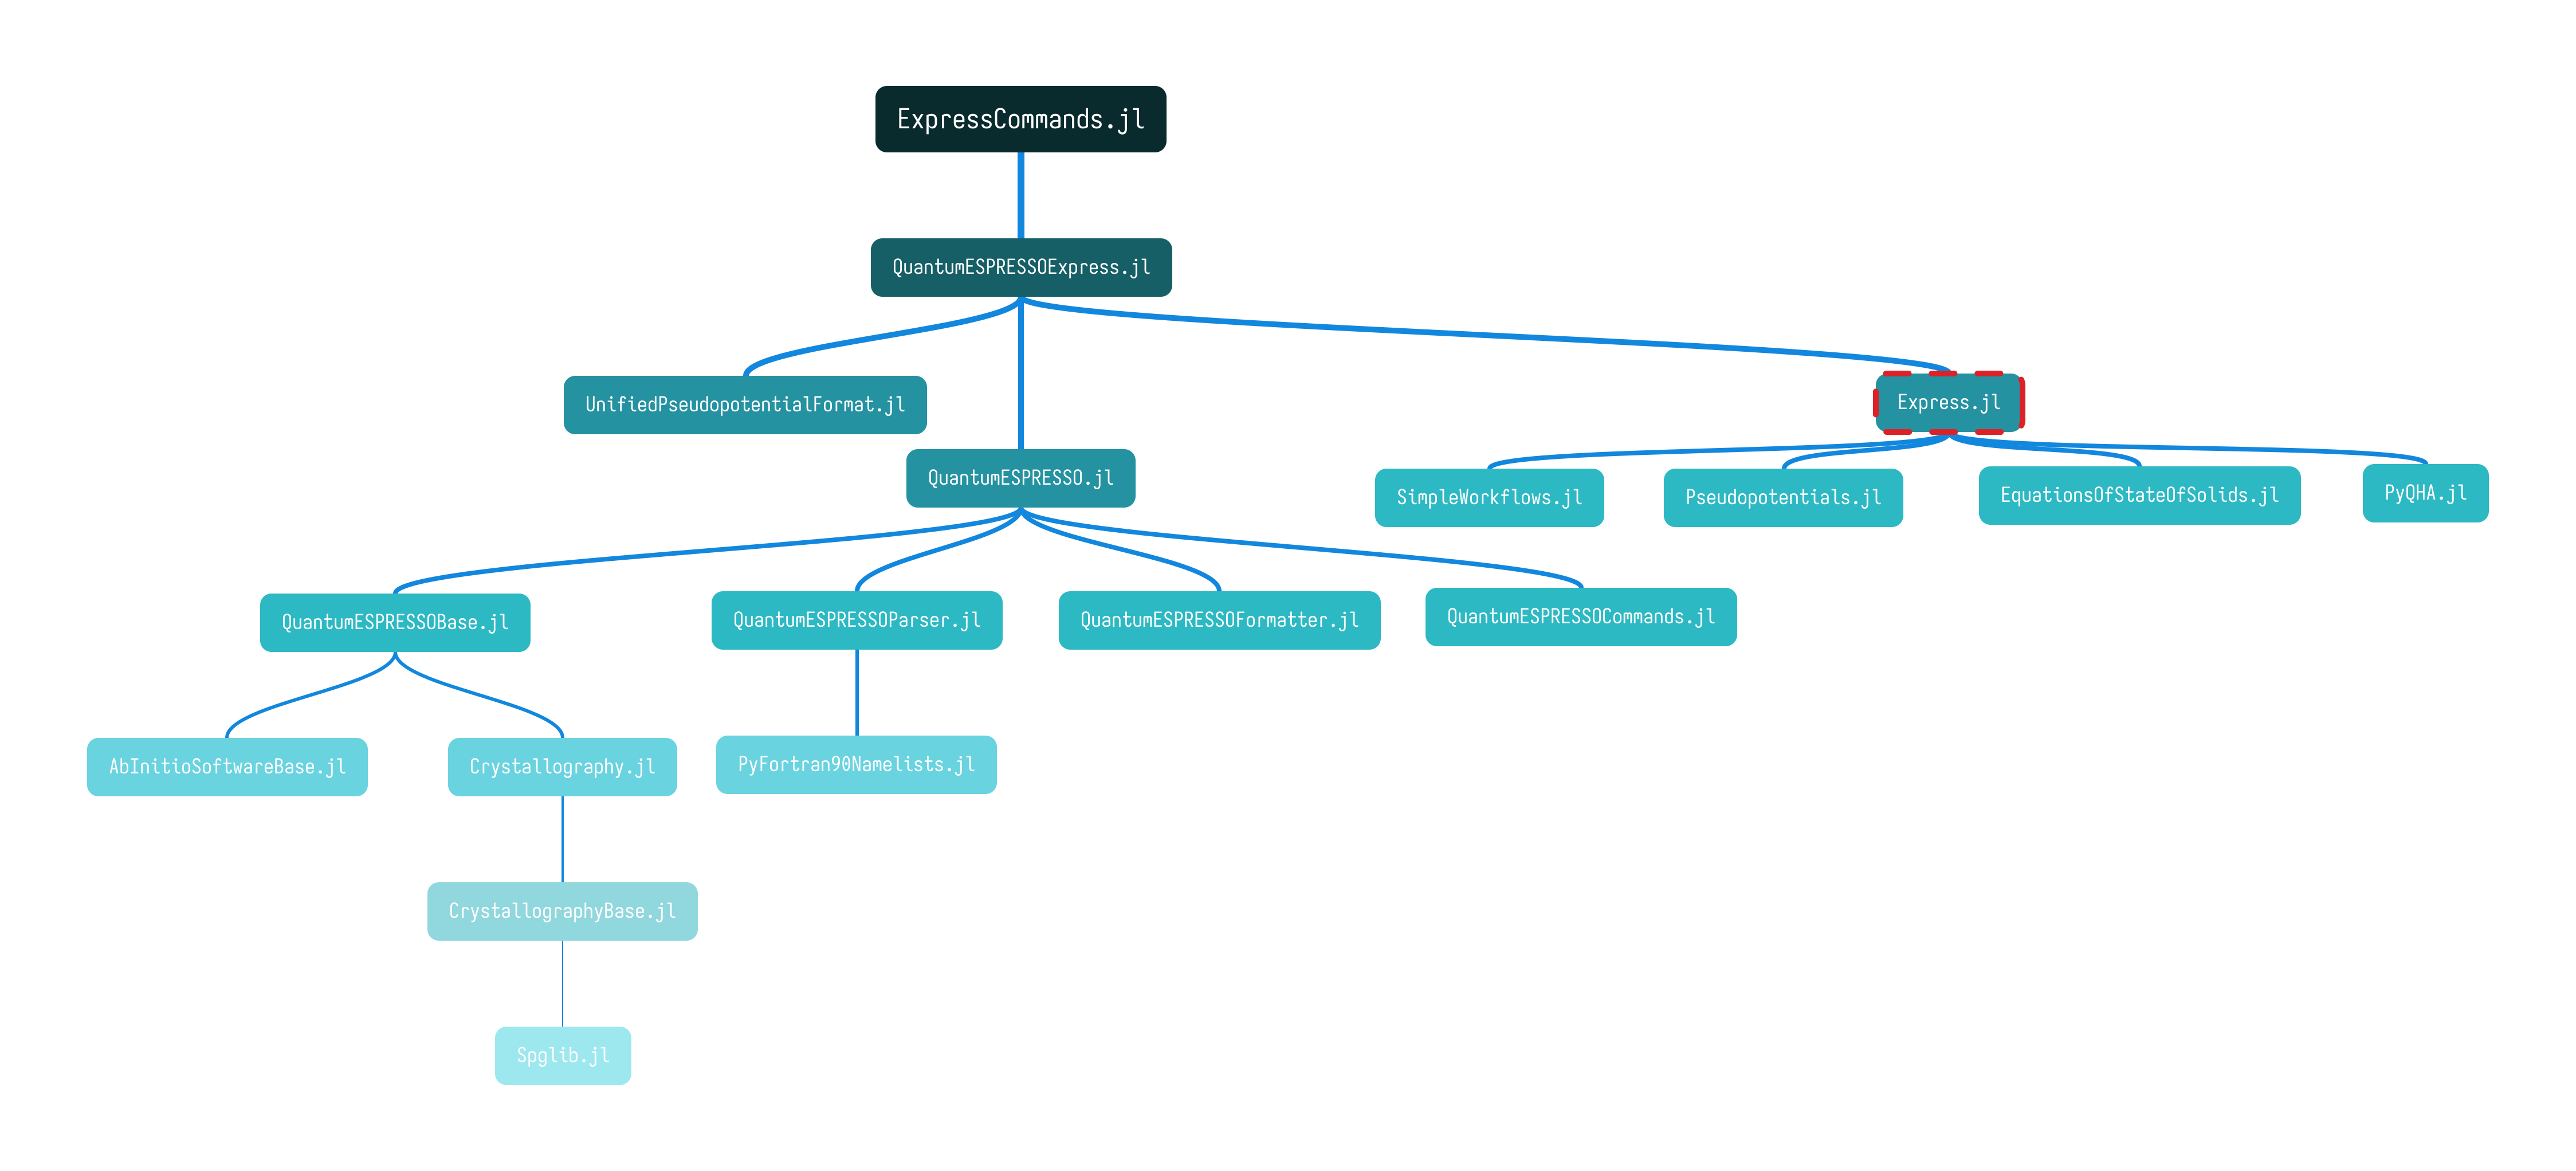
\includegraphics[width=\textwidth]{components}
        \label{fig:components}
    \end{figure}

    \begin{itemize}
        \item \href{https://github.com/MineralsCloud/Express.jl}{\texttt{Express.jl}}
              provides a high-level interface to all the
              workflows, including file reading and writing, job
              creation, submission, monitoring, result retrieving, and data
              analysis. To work with specific software, install the corresponding plugin,
              e.g., \texttt{QuantumESPRESSOExpress.jl} for \qe.
        \item \href{https://github.com/MineralsCloud/ExpressCommands.jl}{\texttt{ExpressCommands.jl}}
              is a user-friendly command-line interface of
              \texttt{Express.jl} for non-developers. It installs an executable
              `\texttt{xps}' that can execute code from configuration files provided by users.
        \item \href{https://github.com/MineralsCloud/EquationsOfStateOfSolids.jl}{\texttt{EquationsOfStateOfSolids.jl}}
              fits energy (or pressure) vs. volume results to equations of state,
              etc. These features are repetitively used in the equation of state workflow.
        \item \href{https://github.com/MineralsCloud/Crystallography.jl}{\texttt{Crystallography.jl}}
              calculates a crystal's primitive cell (or supercell) volume from lattice parameters, finds symmetry
              operations and generates high symmetry points in the Brillouin zone, etc.
        \item \href{https://github.com/MineralsCloud/PyQHA.jl}{\texttt{PyQHA.jl}}
              is a Julia wrapper of
              the Python \texttt{qha} package, which can calculate
              several thermodynamic properties of both single- and multi-configuration
              crystalline materials in the framework of quasi-harmonic approximation.
        \item \href{https://github.com/MineralsCloud/Pseudopotentials.jl}{\texttt{Pseudopotentials.jl}} presents
              a database for storing and querying pseudopotentials used in \ab{} calculations.
        \item \href{https://github.com/MineralsCloud/SimpleWorkflows.jl}{\texttt{SimpleWorkflows.jl}}
              is the skeleton of the workflow system, which
              defines building blocks, composition rules, and operation order of workflows.
        \item \href{https://github.com/MineralsCloud/AbInitioSoftwareBase.jl}{\texttt{AbInitio\-Software\-Base.jl}}
              provides a standard API for some popular \ab{} software such as \qe.
        \item \href{https://github.com/MineralsCloud/QuantumESPRESSOBase.jl}{\texttt{Quantum\-ESPRESSO\-Base.jl}}
              declares basic data types and methods
              for manipulating crystal structures, generating input files for \qe,
              error checking before running, etc.
        \item \href{https://github.com/MineralsCloud/QuantumESPRESSOParser.jl}{\texttt{Quantum\-ESPRESSO\-Parser.jl}}
              parses the input or output files of \qe{} to extract and analyze data.
        \item \href{https://github.com/MineralsCloud/QuantumESPRESSOFormatter.jl}{\texttt{Quantum\-ESPRESSO\-Formatter.jl}}
              formats the input files of \qe.
        \item \href{https://github.com/MineralsCloud/QuantumESPRESSOCommands.jl}{\texttt{Quantum\-ESPRESSO\-Commands.jl}}
              is a command-line interface that exports the commands \qe{} uses in a configurable way.
        \item \href{https://github.com/MineralsCloud/QuantumESPRESSO.jl}{\texttt{QuantumESPRESSO.jl}}
              is simply a wrapper of the types, methods, and commands defined in
              \texttt{Quantum\-ESPRESSO\-Base.jl}, \texttt{Quantum\-ESPRESSO\-Parser.jl},
              \texttt{Quantum\-ESPRESSO\-Formatter.jl},
              and \texttt{Quantum\-ESPRESSO\-Commands.jl} under a common namespace.
    \end{itemize}

\end{frame}

\subsubsection{Binary dependencies and foreign function interface}

\begin{frame}{Build an artifact}

    Operations like finding the symmetry of a crystal,
    are very common in \ab{} calculations (usually the first step).
    Therefore, we need a good library to do this.

    There is a C library called \href{https://github.com/spglib/spglib}{\texttt{spglib}}
    that does this.
    To take this library in productive use, we need first put it in a container
    (``Artifacts''). Luckily, the amazing Julia community has made it possible:
    \href{https://github.com/JuliaBinaryWrappers/spglib_jll.jl}{\texttt{spglib_jll.jl}}.

\end{frame}

\begin{frame}[fragile]{Foreign function interface}

    \begin{columns}
        \begin{column}{0.3\textwidth}
            Now that we have an artifact that exports the functions of the C library,
            it may still be hard to use since it uses some C data structures and API still which may
            not be idiomatic Julia. Therefore, we need to wrap it with a higher level of APIs:
            \href{https://github.com/singularitti/Spglib.jl}{\texttt{Spglib.jl}} is built based on
            this expectation.
        \end{column}

        \begin{column}{0.7\textwidth}
            {\tiny
                \begin{algorithmblock}
                    \begin{juliaverbatim}
function standardize_cell(
    cell::Cell;  # `Cell` was not defined in the C library
    to_primitive = false,
    no_idealize = false,
    symprec = 1e-5,
)
    @unpack lattice, positions, types = _expand_cell(cell)
    to_primitive = Base.cconvert(Cint, to_primitive)
    no_idealize = Base.cconvert(Cint, no_idealize)
    num_atom = Base.cconvert(Cint, length(types))
    allocations = 4
    _positions = Matrix{Cdouble}(undef, 3, num_atom * allocations)
    _types = Vector{Cint}(undef, num_atom * allocations)
    _positions[:, 1:num_atom] = positions
    _types[1:num_atom] = types
    num_atom_std = ccall(
        (:spg_standardize_cell, libsymspg),
        Cint,
        (Ptr{Cdouble}, Ptr{Cdouble}, Ptr{Cint}, Cint, Cint, Cint, Cdouble),
        lattice,
        _positions,
        _types,
        num_atom,
        to_primitive,
        no_idealize,
        symprec,
    )
    if num_atom_std <= 0
        throw(SpglibError("Cell standardization failed!"))
    end
    return Cell(transpose(lattice), _positions[:, 1:num_atom_std], _types[1:num_atom_std])
end
                    \end{juliaverbatim}
                \end{algorithmblock}
            }
        \end{column}
    \end{columns}

\end{frame}

\begin{frame}[allowframebreaks]{Parsers for \ab{} software input and output}

    This is usually hard since most \ab{} are written in Fortran and Julia does not (?)
    have a Fortran parser...

    \framebreak

    \begin{itemize}
        \item For example, \qe{}'s input adopts the \texttt{Namelist} data structure from
              Fortran, and Julia does not have a parser for that...
        \item I know a Python package called
              \href{https://github.com/marshallward/f90nml}{\texttt{f90nml}}, it works well.
              So it came to me that I might write a Julia package that calls that Python
              code.
        \item Therefore, I wrote a very preliminary package
              \href{https://github.com/singularitti/PyFortran90Namelists.jl}{\texttt{PyFortran90Namelists.jl}}
              since writing a parser is time-consuming for a non-CS student like me.
        \item However, it uses \texttt{PyCall.jl}, so sometimes people have trouble installing
              it if they already have Python installed
              (see \href{https://github.com/JuliaPy/PyCall.jl\#specifying-the-python-version}{``Specifying the Python version''}).
    \end{itemize}

    \framebreak

    For output files, it is even more complicated since they usually do not have a standard
    format, therefore lots of regular expressions need to be used.

    It is extremely tricky and error-prone. If you are not familiar with regular expressions,
    try \href{https://github.com/jkrumbiegel/ReadableRegex.jl}{\texttt{ReadableRegex.jl}} to help you build them.

\end{frame}

\begin{frame}[fragile, allowframebreaks]{A wrapper for \ab{} software executables}

    To run external \ab{} software within Julia, what should we do?

    Use the Julia \texttt{AbstractCmd}s? Good choice! But sometimes we want to dynamically generate
    a series of \texttt{AbstractCmd}s. Writing them one by one is not so efficient.

    Or, can we write functions to generate \texttt{AbstractCmd}s? Then all the command
    arguments will be standard Julia function arguments. For example,

    {\scriptsize
            \begin{algorithmblock}
                mpirun -np 16 pw.x -npool 2 -nk 2 -input scf.in > scf.out
            \end{algorithmblock}
        }

    will be

        {\scriptsize
            \begin{algorithmblock}
                \begin{juliaverbatim}
pw("scf.in", "scf.out"; np = 16, npool = 2, nk = 2)
                \end{juliaverbatim}
            \end{algorithmblock}
        }

    \framebreak

    What's more, we could use
    \href{https://github.com/comonicon/Comonicon.jl}{\texttt{Comonicon.jl}},
    to build new executables that will provide customized arguments
    (see \href{https://github.com/MineralsCloud/QuantumESPRESSOCommands.jl}{\texttt{QuantumESPRESSOCommands.jl}})

    {\scriptsize
            \begin{algorithmblock}
                \begin{juliaverbatim}
@cast function pw(input, output = mktemp(parentdir(input))[1]; 
                  np = 1, npool = 1, nk = 1, path = "pw.x", chdir = false)
    ...
    return run(cmd)
end
                \end{juliaverbatim}
            \end{algorithmblock}
        }

    Therefore, we could run it with

        {\scriptsize
            \begin{algorithmblock}
                pw -np 16 -npool 2 -nk 2 -input scf.in scf.out
            \end{algorithmblock}
        }

\end{frame}
